% Phase Portrait for Simple Pendulum
% TikZ diagram for Chapter 2

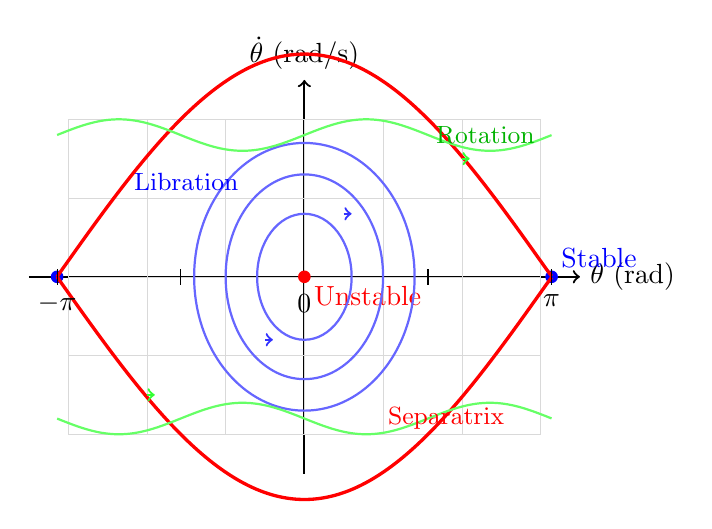
\begin{tikzpicture}[scale=1.0]
    % Axes
    \draw[->, thick] (-3.5, 0) -- (3.5, 0) node[right] {$\theta$ (rad)};
    \draw[->, thick] (0, -2.5) -- (0, 2.5) node[above] {$\dot{\theta}$ (rad/s)};

    % Grid
    \draw[gray!30, very thin] (-3, -2) grid (3, 2);

    % Equilibrium points
    \fill[red] (0, 0) circle (0.08) node[below right] {Unstable};
    \fill[blue] (-3.14, 0) circle (0.08);
    \fill[blue] (3.14, 0) circle (0.08) node[above right] {Stable};

    % Separatrix (homoclinic orbit)
    \draw[red, very thick, domain=-3.14:3.14, samples=100, smooth]
        plot ({\x}, {2*sqrt(abs(cos(\x r) - cos(3.14 r)))});
    \draw[red, very thick, domain=-3.14:3.14, samples=100, smooth]
        plot ({\x}, {-2*sqrt(abs(cos(\x r) - cos(3.14 r)))});

    % Closed orbits (libration) - simplified elliptical approximations
    \draw[blue!60, thick] (0, 0) ellipse (0.6 and 0.8);
    \draw[blue!60, thick] (0, 0) ellipse (1.0 and 1.3);
    \draw[blue!60, thick] (0, 0) ellipse (1.4 and 1.7);

    % Rotation trajectories (outside separatrix) - wavy lines
    \draw[green!60, thick, samples=80, smooth, domain=-3.14:3.14]
        plot ({\x}, {1.8 + 0.2*sin(2*\x r)});
    \draw[green!60, thick, samples=80, smooth, domain=-3.14:3.14]
        plot ({\x}, {-1.8 - 0.2*sin(2*\x r)});

    % Direction arrows
    \draw[->, thick, blue!80] (0.5, 0.8) -- (0.6, 0.8);
    \draw[->, thick, blue!80] (-0.5, -0.8) -- (-0.4, -0.8);
    \draw[->, thick, green!80] (2, 1.5) -- (2.1, 1.5);
    \draw[->, thick, green!80] (-2, -1.5) -- (-1.9, -1.5);

    % Labels
    \node[blue] at (-1.5, 1.2) {\small Libration};
    \node[green!70!black] at (2.3, 1.8) {\small Rotation};
    \node[red] at (1.8, -1.8) {\small Separatrix};

    % Tick marks
    \foreach \x in {-3.14, -1.57, 1.57, 3.14}
        \draw (\x, -0.1) -- (\x, 0.1);
    \node[below] at (-3.14, -0.1) {$-\pi$};
    \node[below] at (3.14, -0.1) {$\pi$};
    \node[below] at (0, -0.1) {$0$};

\end{tikzpicture}
